\noindent
\section{Mapping temporal network to time series}
\label{mapping}
%In this section we describe how we transform a temporal network to a set of time series representing it. 

\begin{figure}
 \begin{center}
 \includegraphics*[width=0.7\columnwidth, angle=0]{./texfiles/Chapter_1/fig/Presentation_d-eps-converted-to.pdf}
 \caption{\label{chap_1_fig1}Converting temporal network to time series}
 \end{center}
 \end{figure}

 We consider a temporal network as a set of static snapshots collected at consecutive time intervals. 
%In this way a temporal graph can be represented as series of static graphs. 
Each snapshot is then represented in terms of eight (mainly structural) properties of the underlying graph. 
 Consequently, we obtain a set of points ordered in time or equivalently a discrete time series (see figure ~\ref{chap_1_fig1}). 
The eight properties we use to represent the temporal network as a time series are:
 
 \begin{itemize} 
  \item (1). {\bf  Number of active nodes}: This is the count of the number of nodes in the system at a given time step. We consider active nodes to be those which have non-zero degree in a time step. We represent the number of active nodes in the system at time step {$t$} by {$N_{t}$}.
  In a similar way we define (2). {\bf number of active edges} and (3). {\bf average degree} and represent the values of these properties at time $t$ by $E_t$ and $Avg\_deg_{t}$ respectively.
  %\item {\bf Average degree}: This is the average degree of the network snapshot at a given time step. We represent average degree at time instance {\large$t$} by 
  %{$Avg\_deg_{t}$}. 
  %\begin{center}
   %{$Avg\_deg_{t}$}={$\frac{2 \times E_{t}}{N_{t}}$}
  %\end{center}

%   \item {\bf Betweenness centrality}: Betweenness centrality of a node is 
%   equal to the number of shortest paths from all vertices to all others that pass through that node.
%   We measure betweenness centrality, represented by {$Bet\_cen_{t}$} of the network snapshot at a given time step {$t$} as the average of the 
%   the betweenness centrality values of the active nodes in the network at $t$.
%   \item {\bf Closeness centrality}: Closeness centrality of a node is the mean distance of that node to all other nodes in the network. 
%     We measure closeness centrality, represented by {$Clos\_cen_{t}$} of the network snapshot at a given time step {$t$} as the average of the 
%   the closeness centrality values of the active nodes in the network at $t$.
%   \item {\bf Clustering coefficient}: We calculate the average clustering coefficient of the active nodes
%   of the network snapshot at a given time step. We represent the average clustering 
%   coefficient at a given time step {$t$} by {$Cluster\_coeff_{t}$}.
\begin{figure}[h]
 \begin{center}
 
 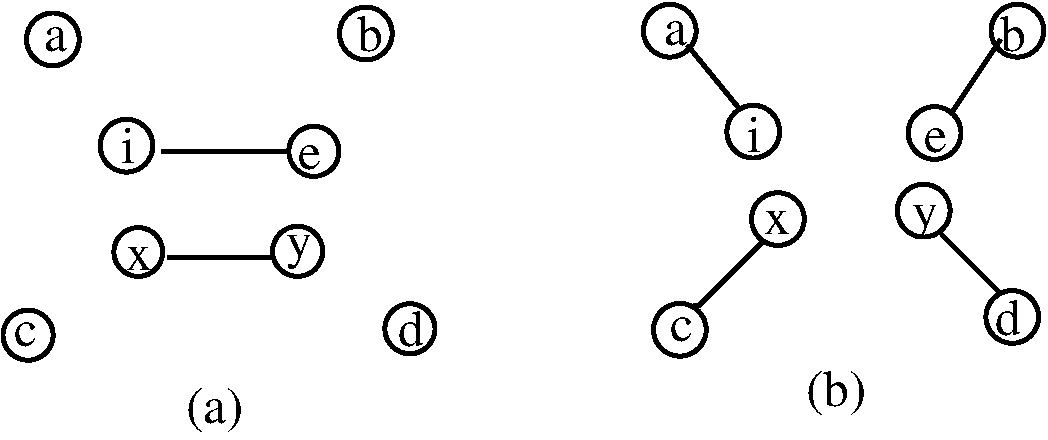
\includegraphics[width=0.7\columnwidth, angle=0]{./texfiles/Chapter_1/fig/ede_em-eps-converted-to.pdf}
 \caption{\label{chap_1_fig3}(a) and (b) denote the status of the network at time $t$ and $t+1$ respectively. For the edge $(i,e)$ in $t$ the corresponding edges
 emanating from $i$ and $e$ are $(i,a)$ and $(e,b)$. For the edge $(x,y)$ they are $(x,c)$ and $(y,d)$. So the $Edge\_emer_{t}=\frac{2+2}{2}=\frac{4}{2}$}
 
%  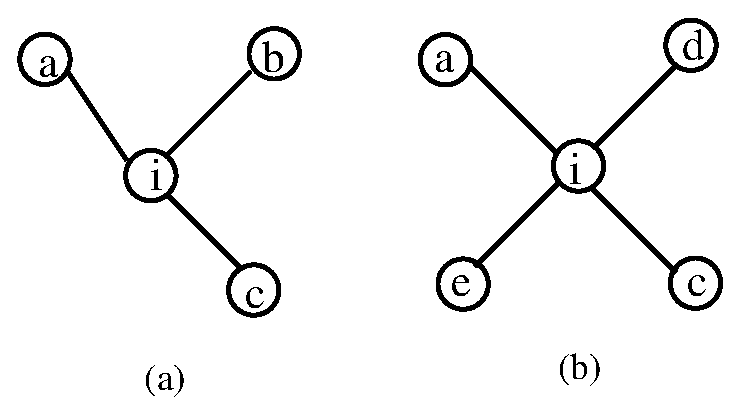
\includegraphics[width=0.8\columnwidth, angle=0]{fig/jaccard.eps}
%  \caption{\label{fig2}(a) and (b) denote the status of node $i$ at time $t$ and $t+k$ respectively. $NBR(i)_{t}=\{a,b,c\}$ and $NBR(i)_{t+k}=\{a,d,c,e\}$ 
%  $Correlation(i)_{k}$={\large$\frac{NBR(i)_{t}\bigcap NBR(i)_{t+k}}{NBR(i)_{t}\bigcup NBR(i)_{t+k}}$}={\large$\frac{2}{5}$} where $NBR(i)_{t}\rightarrow$ the set of neighbors of $i$ at time $t$}
%   
%    \includegraphics[width=0.9\columnwidth, angle=0]{fig/aging_inf2006.eps}
%  \caption{\label{aging}The value of the correlation decreases as we increase the lag between the network snapshots (INFOCOM 2006 dataset). The $X$ axis represents lag and $Y$ axis
%   represents the average correlation value.\vspace{-6mm}}
  
 
 \end{center}
 \end{figure}

   
\item (4). {\bf  Edge emergence}: Edge emergence ~\cite{sur2014attack} is a measure that estimates structural similarity. For measuring the 
  edge emergence at time $t$ we consider each edge of the network at time $t$ and for each of its two endpoints we calculate the number of edges 
  emerging in the next time step $t+1$. We represent edge-emergence at time $t$ by $Edge\_emg_{t}$. If $E_t$ denotes the set of edges present in the network at time $t$ 
  and $A_{t+1}$ denotes the set of edges at time $t+1$ which are adjacent to $E_t$ then $Edge\_emg_{t}=\frac{|A_{t+1}|}{|E_{t}|}$. 
Figure~\ref{chap_1_fig3} shows how we calculate this measure for a temporal network at any time instance.
  
  
  \item (5). {\bf  Modularity}: We decompose each snapshot into communities using the technique specified in ~\cite{blondel2008fast}
  and measure the goodness of this division using modularity ~\cite{newman2006modularity}. We represent modularity 
  of the system at a given time step {$t$} by {$Mod_{t}$}. 
  
%   We also consider {\bf betweenness centrality}, {\bf closeness centrality} and {\bf clustering coefficient} and their values at time step $t$ are represented by 
%   {$Bet\_cen_{t}$}, {$Clos\_cen_{t}$} and {$Cluster\_coeff_{t}$} respectively.
  
 \end{itemize}
 We also consider (6). {\bf  betweenness centrality}, (7). {\bf closeness centrality} and (8). {\bf  clustering coefficient} of the graph (values computed for each node and then summed over all nodes); their values at time step $t$ are represented by 
  {$Bet\_cen_{t}$}, {$Clos\_cen_{t}$} and {$Clus\_coeff_{t}$} respectively.

\medskip
